\section{\textsc{Gewienertes Omelett}}

\subsection*{Zutaten für 2 Omelettes:}

\begin{tabular}{p{7.5cm} p{7.5cm}}
	& \\
	8 Eier & 4 Wiener Würstchen \\
	1 Zwiebel & 400g Mozzarella \\
	Salz \& Pfeffer &
\end{tabular}

\subsection*{Serviervorschlag:}

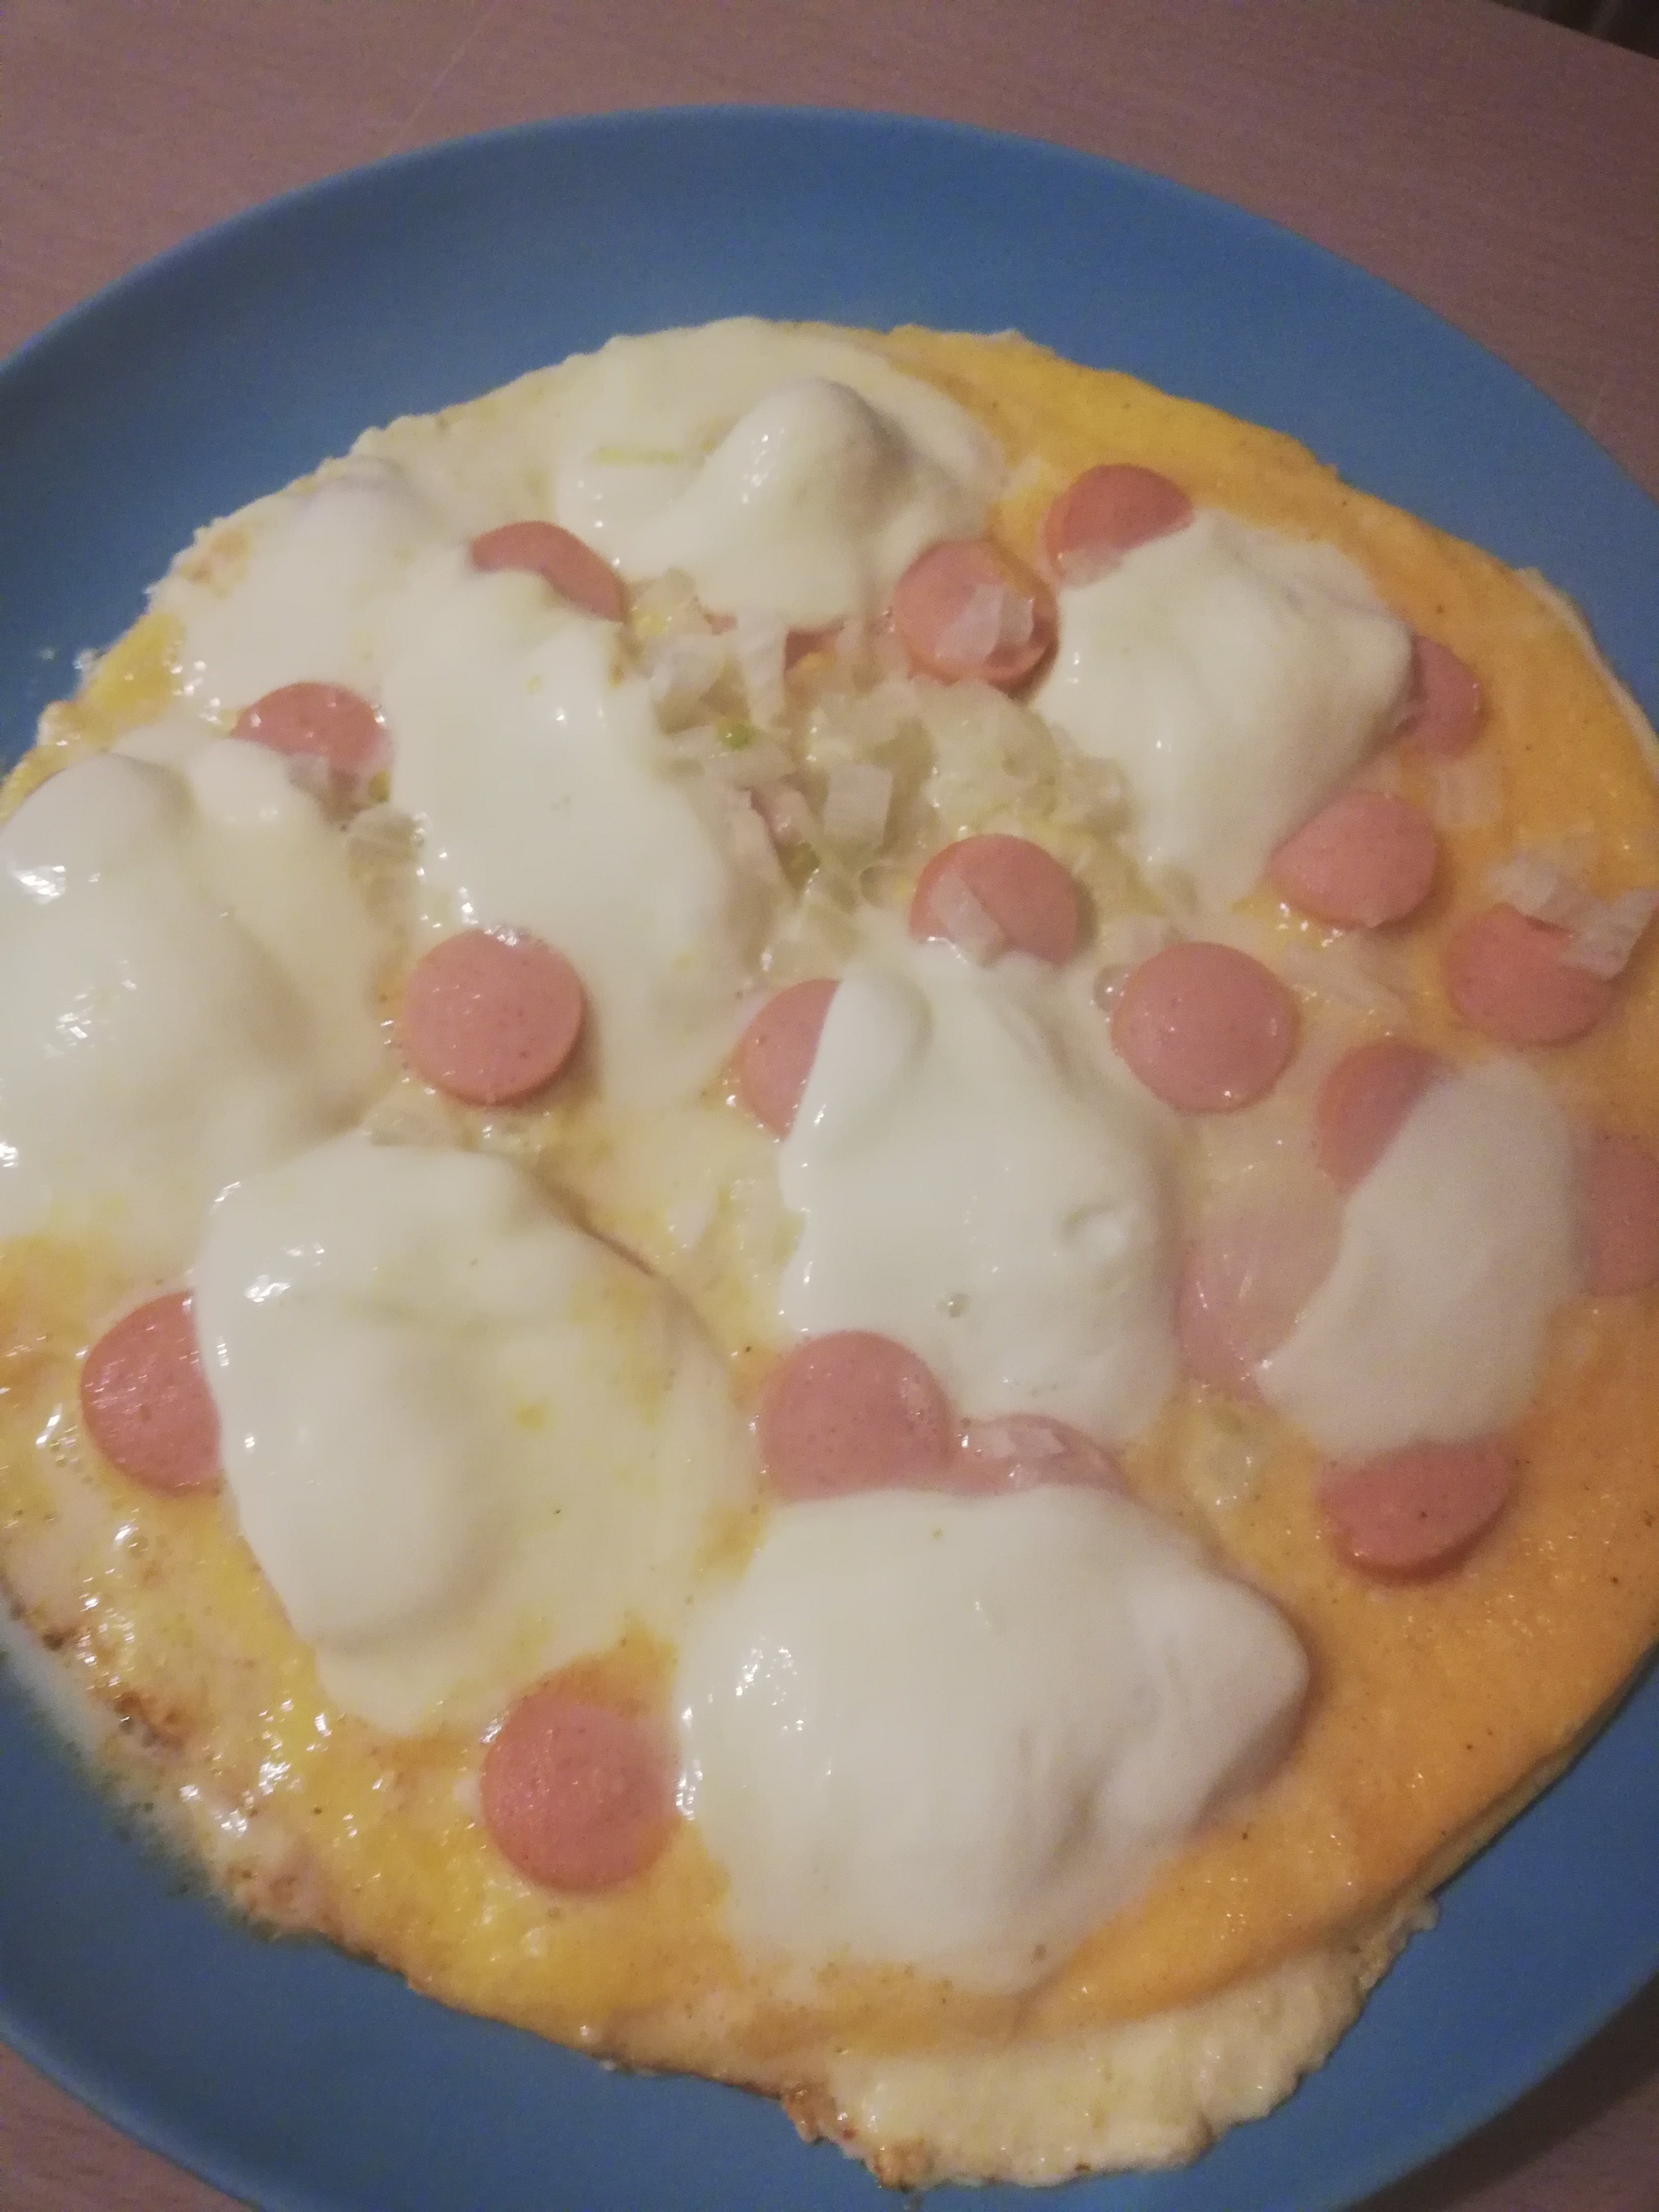
\includegraphics[width=\textwidth]{img/omlett/omlett_wiener_fertig.jpg} \cite{omlettwiener}

\subsection*{So geht's}

\begin{tabular}{p{15cm}}
	Die Eier in eine Schüssel aufschlagen und schaumig schlagen.\\
	Butter in einer großen Pfanne schmelzen.\\
	In der Zwischenzeit die Wiener in dünne Scheiben schneiden.\\
	Die Zwiebeln fein würfeln.\\
	Die Eimasse in die Pfanne geben und auf großer Hitze stocken lassen.\\
	Die Wiener und die Zwiebeln auf dem Omelett verteilen.\\
	Mit einem Deckel auf der Pfanne 5min braten.\\
	Auf einem großen Teller servieren.
\end{tabular}
